\documentclass[11pt]{article}

\let\counterwithout\relax
\let\counterwithin\relax

\usepackage{amsmath, amsfonts, amssymb, amsthm, bm, graphicx, mathtools, enumerate,multirow}
%\usepackage[affil-it]{authblk}
\usepackage{natbib}
\usepackage[CJKbookmarks=true,
bookmarksnumbered=true,
bookmarksopen=true,
colorlinks=true,
citecolor=blue,
linkcolor=blue,
anchorcolor=blue,
urlcolor=blue]{hyperref}
% \usepackage{hyperref}
\usepackage[usenames]{color}
\usepackage[letterpaper, left=1.2truein, right=1.2truein, top = 1.2truein,
bottom = 1.2truein]{geometry}
\usepackage[ruled, lined, commentsnumbered]{algorithm2e}
\usepackage{prettyref,soul}

\usepackage{apptools} %Ya
%\usepackage{enumitem} %Ya
\usepackage{chngcntr} % define \counterwithin
\AtAppendix{\counterwithin{lemma}{section}} %Ya
\usepackage{tikz}
\usepackage[font=small,labelfont=bf]{caption}
\usepackage{enumitem}



\newtheorem{lemma}{Lemma}
\newtheorem{proposition}{Proposition}
\newtheorem{thm}{Theorem}
\newtheorem{definition}{Definition}
\newtheorem{corollary}{Corollary}
\newtheorem{assumption}{Assumption}
\theoremstyle{definition}
\newtheorem{remark}{Remark}


\newrefformat{eq}{(\ref{#1})}
\newrefformat{chap}{Chapter~\ref{#1}}
\newrefformat{sec}{Section~\ref{#1}}
\newrefformat{algo}{Algorithm~\ref{#1}}
\newrefformat{fig}{Fig.~\ref{#1}}
\newrefformat{tab}{Table~\ref{#1}}
\newrefformat{rmk}{Remark~\ref{#1}}
\newrefformat{clm}{Claim~\ref{#1}}
\newrefformat{def}{Definition~\ref{#1}}
\newrefformat{cor}{Corollary~\ref{#1}}
\newrefformat{lmm}{Lemma~\ref{#1}}
\newrefformat{lemma}{Lemma~\ref{#1}}
\newrefformat{prop}{Proposition~\ref{#1}}
\newrefformat{app}{Appendix~\ref{#1}}
\newrefformat{ex}{Example~\ref{#1}}
\newrefformat{cond}{Condition~\ref{#1}}



\def\pr{\mathbb{P}} % the symbol P for probability used the sans serif letter
\def\E{\mathbb{E}} % the symbol E for expectation used the sans serif letter
\def\Cov{\mathrm{Cov}} % the symbol Cov for covariance used the sans serif letter
\def\Var{\mathrm{Var}} % the symbol Var for covariance used the sans serif letter
\def\vec{\mathrm{vec}} % the symbol Var for covariance used the sans serif letter


\newcommand{\tp}{\intercal}
\newcommand{\brm}[1]{\bm{\mathrm{#1}}}
\newcommand{\bigO}{\ensuremath{\mathop{}\mathopen{}\mathcal{O}\mathopen{}}}
\newcommand{\smallO}{ \scalebox{0.7}{$\mathcal{O}$}}
\newcommand{\bigOp}{\bigO_\mathrm{p}}
\newcommand{\smallOp}{\smallO_\mathrm{p}}
\newcommand{\R}{\mathbb{R}}
\newcommand{\balpha}{\bm{\alpha}}
\newcommand{\bbeta}{\bm{\beta}}
\newcommand{\btheta}{\bm{\theta}}
\newcommand{\bX}{\brm{X}}
\newcommand{\bB}{\brm{B}}

\newcommand{\argmin}{\ensuremath{\operatornamewithlimits{arg\,min}}}
\newcommand{\BNTR}{BroadcasTR}
%\newcommand{\supp}[1]{{\bf\textcolor{red}{#1}}}

%\newcommand{\hh}[1]{{\bf\textcolor{red}{[hl: #1]}}}
\newcommand{\hh}[1]{{\bf\textcolor{red}{#1}}}
%%%%%%%%%%
%
\newcommand{\ya}[1]{{\bf\textcolor{cyan}{[Ya: #1]}}}
%\newcommand{\supp}[1]{{\bf\textcolor{red}{#1}}}
\newcommand{\supp}[1]{#1}


%%%%%%%ya for unpenalized and penalized \hat{m}
\newcommand{\LS}{\rm LS}
\newcommand{\PLS}{\rm PLS}


\newcommand{\revise}[1]{\textcolor{blue}{#1}}
\newenvironment{revise_block}{\color{blue}}{}


\usepackage[T1]{fontenc}
\usepackage[utf8]{inputenc}
\usepackage{authblk}
%\title{Masked Modeling for ECG}
%\title{Masked Electrocardiograph Transformer for multi-label Classification}
\title{ECG2HCM}

%\author[1,\#,*]{Ya Zhou}
%\author[1,\#]{Xiaolin Diao}
%\author[1]{Yanni Huo}
%\author[1]{Yang Liu}
%\author[2,*]{Xiaohan Fan}
%\author[3,*,\dag]{Wei Zhao}
%\affil[1]{Department of Information Center, Fuwai Hospital, Chinese Academy of Medical Sciences and Peking Union Medical College, Beijing, 100037, China}
%\affil[2]{%State Key Laboratory of Cardiovascular Disease, 
%	%Cardiac Arrhythmia Center, Fuwai Hospital, National Center for Cardiovascular Diseases, Chinese Academy of Medical Sciences and Peking Union Medical College, Beijing, 
%	Cardiac Arrhythmia Center, Fuwai Hospital, National Center for Cardiovascular Diseases, Chinese Academy of Medical Sciences and Peking Union Medical College, Beijing, 
%	China,  100037, China}
%\affil[3]{Fuwai Hospital, National Center for Cardiovascular Diseases, Chinese Academy of Medical Sciences and Peking Union Medical College, Beijing, 100037, China}

\renewcommand*{\Affilfont}{\small\it}
\renewcommand\Authands{ and }
\date{}

\begin{document}
\maketitle
%\def\thefootnote{\#}\footnotetext{The authors  }
%\def\thefootnote{\arabic{footnote}}
%\def\thefootnote{*}\footnotetext{Corresponding authors: Ya Zhou (zhouya@fuwai.com), Xiaohan Fan (fanxiaohan@fuwaihospital.org), Wei Zhao (zw@fuwai.com) }\def\thefootnote{\arabic{footnote}}
%\def\thefootnote{ \dag}\footnotetext{Supervision: Wei Zhao}


\begin{abstract}
test
\end{abstract}
Keywords: 

\section*{Introduction}
\label{sec:intro}

\subsection*{AI technique, for reference}
Several Convolutional Neural Networks (CNN) have been utilized for detecting Hypertrophic Cardiomyopathy (HCM) from Electrocardiogram (ECG) data \citep{ko2020detection, goto2022multinational, siontis2023saliency,  siontis2024hypertrophic}. While CNN excel at extracting local information, their limited local receptive field in the convolution operation constrains their capability to capture global information \citep{song2022ctmfnet, yang2021transformer}. In contrast, Transformer has emerged as a promising alternative, leveraging innate global self-attention mechanisms to model long-range dependencies \citep{vaswani2017attention, dosovitskiy2020image}. Numerous empirical studies have demonstrated that Transformer-based models with self-supervised pre-training outperform their CNN counterparts across various vision tasks \citep{matsoukas2021time}. For traditional ECG interpretations, we have proposed a self-supervised Transformer-based method, which significantly enhances macro F1 scores by 9.9\% to 32.0\% on the publicly available PTB-XL dataset, compared to many state-of-the-art algorithms \citep{wagner2020ptb, zhou2023masked}. 
In this study, we adopt this method within a multi-task architecture to detect the HCM and its subgroups, and evaluate the performance on a large Chinese dataset. 



\section*{Method}
\label{sec:method}

%We developed a Transformer-based algorithm based on the method proposed in a recent study. Briefly,  our approach follows the pretrain-and-finetune paradigm, as shown in Figure 1. During pre-training, the model is an encoder-decoder network, with the same setting as MTECG-T presented in the previous study. Specifically, the encoder comprises a linear projection, a positional embedding, and 12 Transformer blocks with a self-attention head of 3 and a latent dimension of 192. The decoder consists of a linear projection, a positional embedding, and a single-layer Transformer with a self-attention head of 4 and a latent dimension of 128. To process the $12 \times 5000$ ECG signal, we split it into 200 non-overlapping segments along the time dimension. The ECG segments are randomly uniformly divided into masked segments and unmasked segments with a ratio of 2.5: 7.5. 
%The pre-training objective is to reconstruct the per-segments normalization of the masked segments by using the unmasked segments.  To enhance the model's generalization capabilities, we pre-train the model 1600 epochs, with the default hyperparameters of MTECG-T, using a combination of the labeled training dataset and unlabeled data, as illustrated in Figure 1(A). 


%aim to evaluate the performance of advanced AI techniques in the detection of HCM based on 12-lead ECG data from a large Chinese dataset.  Additionally,  we will adopt a multi-task architecture to provide the model with additional information from the label hierarchy of HCM and its subgroups. 


%
%Several Convolutional Neural Networks (CNN) have been adopted to detect HCM from ECG data. Although CNN are good at extracting local information, the local receptive filed of the convolution operation limits the network’s ability to extract global  information \citep{song2022ctmfnet, yang2021transformer}.  Transformer has emerged as an alternative with innate global self-attention mechanisms to capture long-range dependencies \citep{vaswani2017attention, dosovitskiy2020image}. Many empirical studies found that Transformer-based models with self-supervised pre-training outperforms their CNN counterparts in many tasks \citep{matsoukas2021time}. We have proposed an self-supervised Transformer-based methods for ECG classification, which increases the macro F1 scores by 9.9\%-32.0\% on the publicly available PTB-XL dataset \citep{wagner2020ptb} for ECG diagnosis, compared to many state-of-the-art algorithms \citep{zhou2023masked}. In this study, we will test the advanced AI technique in detection of HCM based on the 12-lead ECG in a large Chinese dataset. In addition, we will adopt a multi-task architecture to give the model additional information from the label hierarchy of HCM and its subgroups. 

%Considering the there exits 

%However, the mechanism of convolution operation limit the network’s ability to extract global  information.

%exhibits limitations in modeling long-range relations


\subsection*{Model development}

\begin{figure}[!hbt]
	\centering
	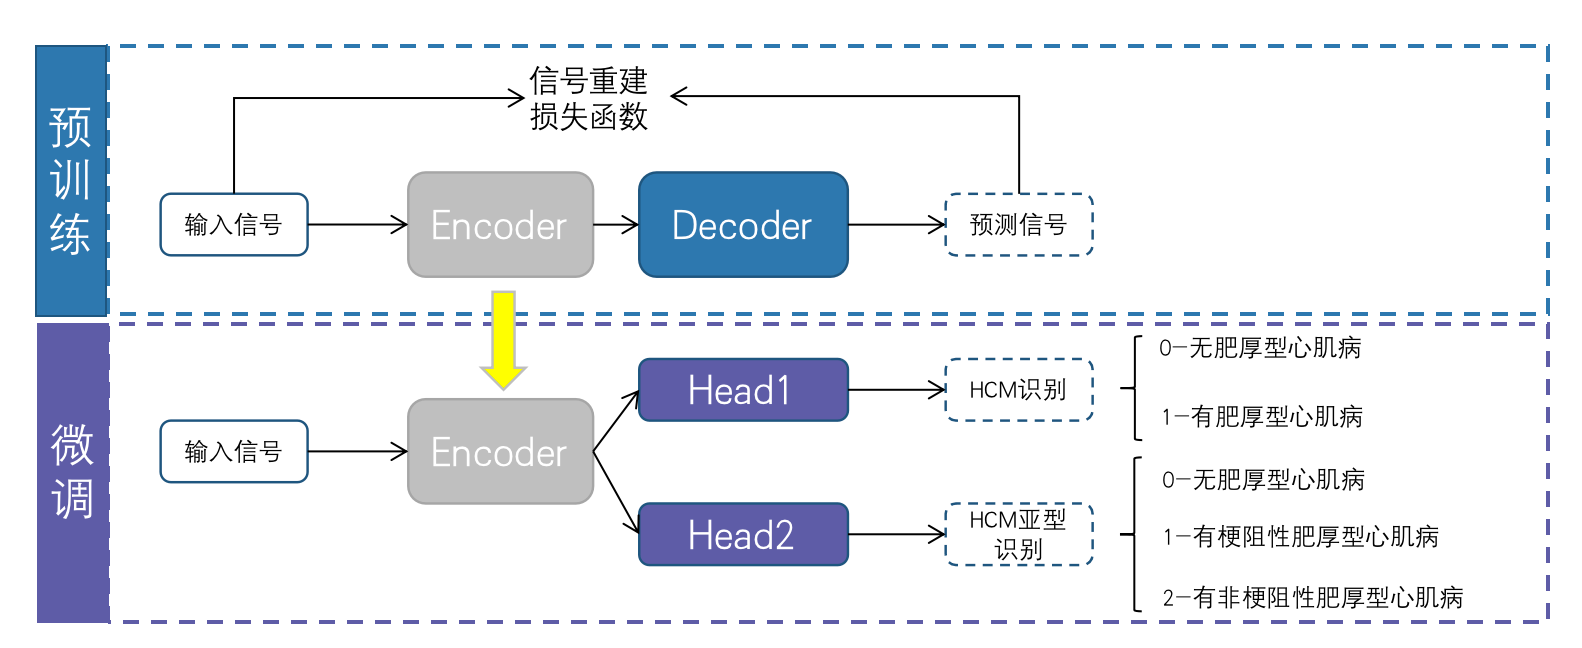
\includegraphics[width = 150 mm %, height = 10 mm
	]{./model_achi}
	\caption{model architecture
		\label{model_achi} }
\end{figure}

We developed a Transformer-based algorithm based on a masked modeling method proposed in a recent study \citep{zhou2023masked}. Briefly, our approach follows the pretrain-and-finetune paradigm, as shown in Figure \ref{model_achi}. During pre-training, the model is an encoder-decoder network, with the same setting as MTECG-T, presented in the previous study \citep{zhou2023masked}. The encoder comprises a linear projection, a positional embedding, and 12 Transformer blocks with 3 self-attention heads and 192 latent dimension. The decoder consists of a linear projection, a positional embedding, and a 1-layer Transformer with 4 self-attention heads and 128 latent dimension. To handle the $12 \times 5000$ ECG signal, we split it into 200 non-overlapping segments along the time dimension, and uniformly randomly divide them into masked segments and unmasked segments with a ratio of 2.5: 7.5. The pre-training objective is to reconstruct the per-segments normalization of the masked segments using the unmasked segments. To enhance the model's generalization capabilities, we pre-train the model for 1600 epochs, with the default hyperparameters of MTECG-T, using a combination of the labeled training dataset and unlabeled dataset, as illustrated in Figure \ref{model_achi} (A).

In fine-tuning, we retained the pre-trained encoder and adopted a multi-task architecture, as shown in Figure \ref{model_achi} (B). The first task involves a binary classification to detect HCM, while the second task is a multi-class classification to detect its subtype. For these tasks, we employed the binary cross-entropy loss and the cross-entropy loss, respectively. 
Recent studies suggest that the simple scalarization with uniform weights often performs comparably to more complex multitask methods \citep{royer2024scalarization}. 
Therefore, we directly added the loss functions as the fine-tuning objective. We trained the model for 50 epochs with the default hyperparameters of MTECG-T and saved the model weights in a checkpoint after every epoch. Then, we reverted the model to the checkpoint corresponding to the optimal F1 scores for HCM on the validation set.

%The unmasked segments are feed to the model to reconstruct the  per-segments normalization of the masked segments.  
%and learnable positional embeddings are added after the linear projection layer in both encoder and decoder. Additionally, we employ a masking ratio of 0.25 and adopt a per-segment normalization reconstruction target. 
%To enhance the model's generalization capabilities, we pre-train the model using a combination of the labeled training dataset and unlabeled data, as illustrated in Figure 1(A). 
%




%In fine-tuning, we kept the pre-trained encoder and adopt a multi-task architecture. As shown in Figure 1(B),  the first is a binary classification task to detect HCM and the second is a multi-class classification task to detect its subtype, where we adopted the binary cross entropy and cross entropy loss functions, respectively. Recent studies have shown that simple scalarization with uniform weights actually often performs on-par with other complex multitasks methods. We therefore directly added the loss functions as the fine-tuning objective. We train the model 50 epochs with the default hyperparameters of MTECG-T and saved model weights in a checkpoint for every epoch. We then reverted the model to the checkpoint corresponding to the  optimal F1 scores for HCM on the validation set. 






%as shown in Figure 1 (B).   


%we do not only apply a multi-class classification to detect subtypes of HCM. Instead, we consider an additional binary classfication task to detect if HCM exists in a multi-task architecture. Due to the overlap information for the two tasks, we adopt the hard parameter sharing method, as shown in Figure 1(B). 





%adopted a multi-tasks architecture, where the first task is the detection of HCM and the second task is to distinguish the type, as show in Figure 1(B). Consider 






%the encoder consists by 12 Transformer blocks with a self-attention head of 3 and a latent dimension  of 192, while the decoder is a 1-layer Transformer with a self-attention head of 3 and a latent dimension of 128. 

%the neural network includes 3 parts, i.e., the encoder, decoder and the classification head, as shown in Figure 1. We adopted the setting of MTECG-T presented in the previous study. The encoder consists by 12 Transformer blocks with a self-attention head of 3 and a latent dimension  of 192, while the decoder is a 1-layer Transformer with a self-attention head of 3 and a latent dimension of 128. For the classification head, we consider a multi-task architecture. 





 
 
% method follows the pretrain-and-finetune paradigm and
% 
% 
%
%  consists of 5 majors components including segment operation, mask operation, encoder, decoder, and reconstruction target. We adopted the setting of MTECG-T.  The $12 \times 5000$ ECG signal is split into 200 non-overlapping segments along the time dimension with size 25. The encoder consists by 12 Transformer blocks with a self-attention head of 3 and a latent dimension  of 192, while the decoder is a 1-layer Transformer with a self-attention head of 3 and a latent dimension of 128.
% 
 
 %A uniform masked strategy and per-segment normalization are utilized. 
 
 
% Our model training is similar to the previous study and follows the pretrain-and-finetune paradigm. We pre-train 
% 
%  The pre-training is on the training set associated with those unmatched ECG signals. 



%we adopted MTECG-T as the backbone.   




%The 12 * 5000 ECG signal is split into 200 non-overlapping segments along the time dimension with size 25. The methods 

%We followed the pretrain-and-finetune paradigm by using the suggested hyper-parameters in the aforementioned study. 

%The method consists of 5 major components, segment operation, mask operation, encoder, decoder, and reconstruction target. 
















\bibliographystyle{rss} 
%\bibliographystyle{acm}
\bibliography{reference}




\end{document}
